%==============================================================================%
\section{Smart Street Sensor Project}
%==============================================================================%
The Smart Street Sensor project is one of the most comprehensive studies carried out on consumer volume and characteristics in retail areas across the UK.
The project has been organised as a collaboration between the Consumer Data Research Centre, University College London (CDRC, UCL) and the Local Data Company (LDC).
The project was designed to serve as the first and unique comprehensive research into the patterns of retail activity in high streets of United Kingdom by measuring their real-time footfall from collecting Wi-Fi probe requests.
The data for the project was collected through sensors installed at around 1000 retail locations across UK.

The primary aim of the project is to improve our understanding of the dynamics of the high street retail climate in UK.
As we saw in our literature review, unlike online retail, this involves the quantification and measurement of human activity at small scales, such as high streets, which is already the subject of active research.
The key challenge in this area is the collection of data at the smallest scales possible with minimal resources while not infringing on people’s privacy.
This challenge when solved can provide immense value to the occupiers of the retail premises who want to improve revenues, to landlords who want to increase the value of the property, to local authorities who want to improve the vibrancy of the retail economy, and finally to investors and consumers within the retail industry.
The project also aims to facilitate decision making by these stakeholders, in addition to the tremendous opportunities for academic research.

\begin{marginfigure}[-2cm]
  \centering
  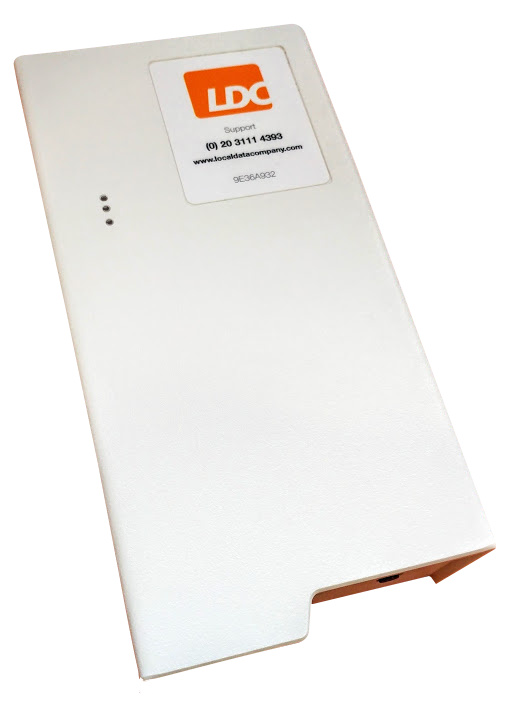
\includegraphics[height=3.5cm]{images/sss-hardware.jpg}
  \caption{Hardware setup used to collect data in the pilot studies.}
  \label{figure:collection:sss:hardware}
\end{marginfigure}

%------------------------------------------------------------------------------%
\subsection{Methodology}
%------------------------------------------------------------------------------%
As a first step, various locations for the study were identified by the CDRC to include a wide geographical spread, different demographic characteristics, and range of retail centre profiles.
Figure \ref{figure:collection:sss:locations} shows all the locations in the United Kingdom city-wise and Table \ref{table:collection:sss:locations} shows the regional distribution of the locations.

\begin{table}
  \footnotesize
  \begin{center} 
    \begin{tabular}{lr} 
      \toprule
      Region & Locations \\
      \midrule
      Greater London & 479 \\
      Scotland & 118 \\
      Yorkshire and the Humber & 114 \\
      South East & 103 \\
      North West & 98 \\
      South West & 87 \\
      East Midlands & 68 \\
      East Of England & 49 \\
      West Midlands & 39 \\
      North East & 26 \\
      Wales & 17 \\
      Northern Ireland & 2 \\
      \bottomrule
    \end{tabular}
  \end{center}
  \caption{Regional distribution of Smart Street Sensor locations across UK}
  \label{table:collection:sss:locations}
\end{table}

\begin{marginfigure}[6cm]
  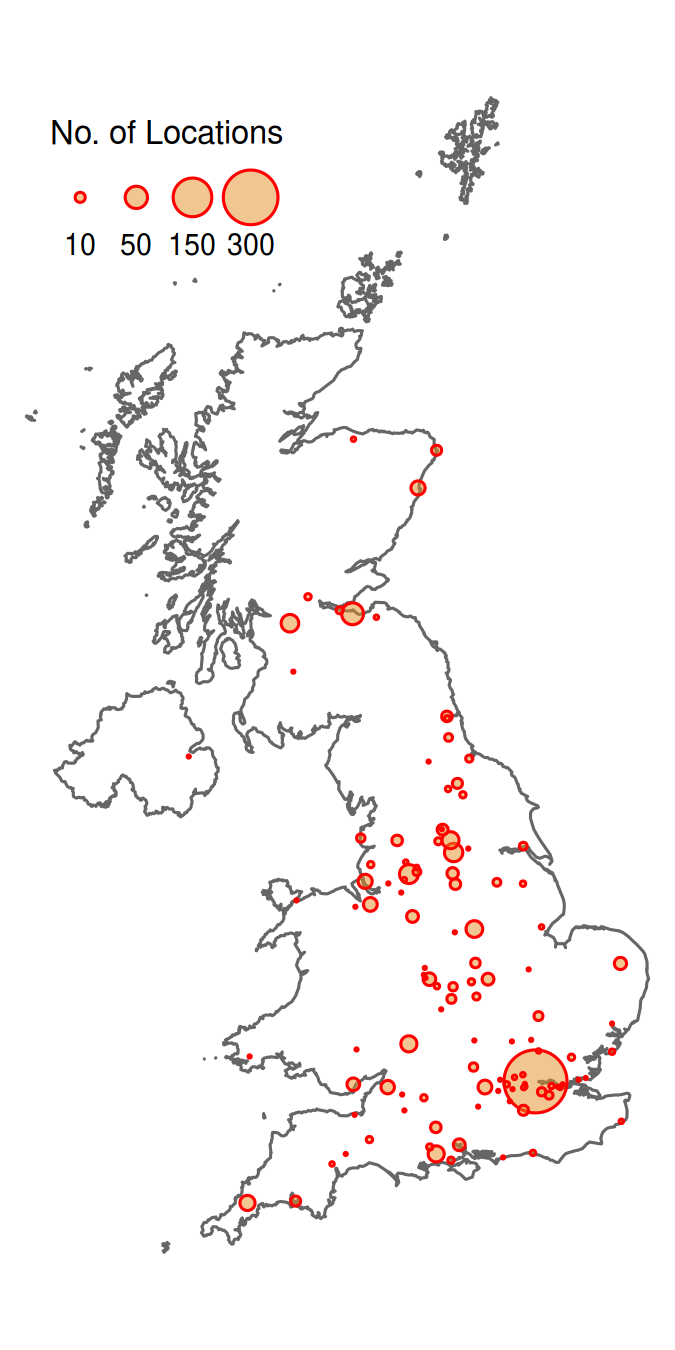
\includegraphics[trim = {0 20 0 0}, clip]{images/sss-locations.png}
  \caption{Distribution of locations with Smart Street Sensors installed.}
  \label{figure:collection:sss:locations}
\end{marginfigure}

We can see that the project has a strong London bias which along with other retail centres in the Greater London area, accounts for almost half of the locations.
We must also note that the locations are retail and any insight from the data needs to be looked at with a retail point of view.

A custom footfall counting technology using Wi-Fi sensors (Figure \ref{figure:collection:sss:hardware}) was also designed and developed by LDC, and the sensors were installed at the identified locations.
The sensor employs proprietary hardware and software, and monitors and records the probe requests sent by Wi-Fi enabled mobile devices present in its range.
In addition to this, the number of people walking by the sensor were counted manually for short time periods during the installation of the sensors at the corresponding locations.
The project aimed to combine these two sets of data to use as a proxy for estimating footfall at these locations.
The potentially personally identifiable information collected on the mobile devices are converted into a unique cryptographic hash at the sensor level and the data is sent to central server via encrypted channel for storage.
This data is then retrieved securely for the preparation of the commercial dashboards by LDC and for research purposes by CDRC.

The sensors are usually installed on a partnering retailer's shop window so that its range covers the pavement in front of the shops.
A typical configuration of a sensor in a location with respect to the premises and the pavement in front of it is illustrated in Figure \ref{figure:collection:sss:typical}.
There are also a small percentage (3\%) of the devices which are installed within large shops to monitor internal footfall.
Each device collects data independently and uploads the collected data to a central microsoft cloud facility (Azure) container at regular intervals of 5 minutes through a dedicated 3G mobile data connection.
The sensor hardware has been improved over the course of the project, and currently has built in failure prevention mechanisms such as, backup battery for power failures, automatic reboot capabilities, and in-device memory for holding data when the internet is not available.
The project began with the first sensor installation in July 2015, and has grown to an average of 650 daily active sensors as of January 2019, with a total of 1200 locations been involved in the project since its inception.
We have collected around 2TB of data comprising of around 73 billion probe requests.

\begin{figure*}
  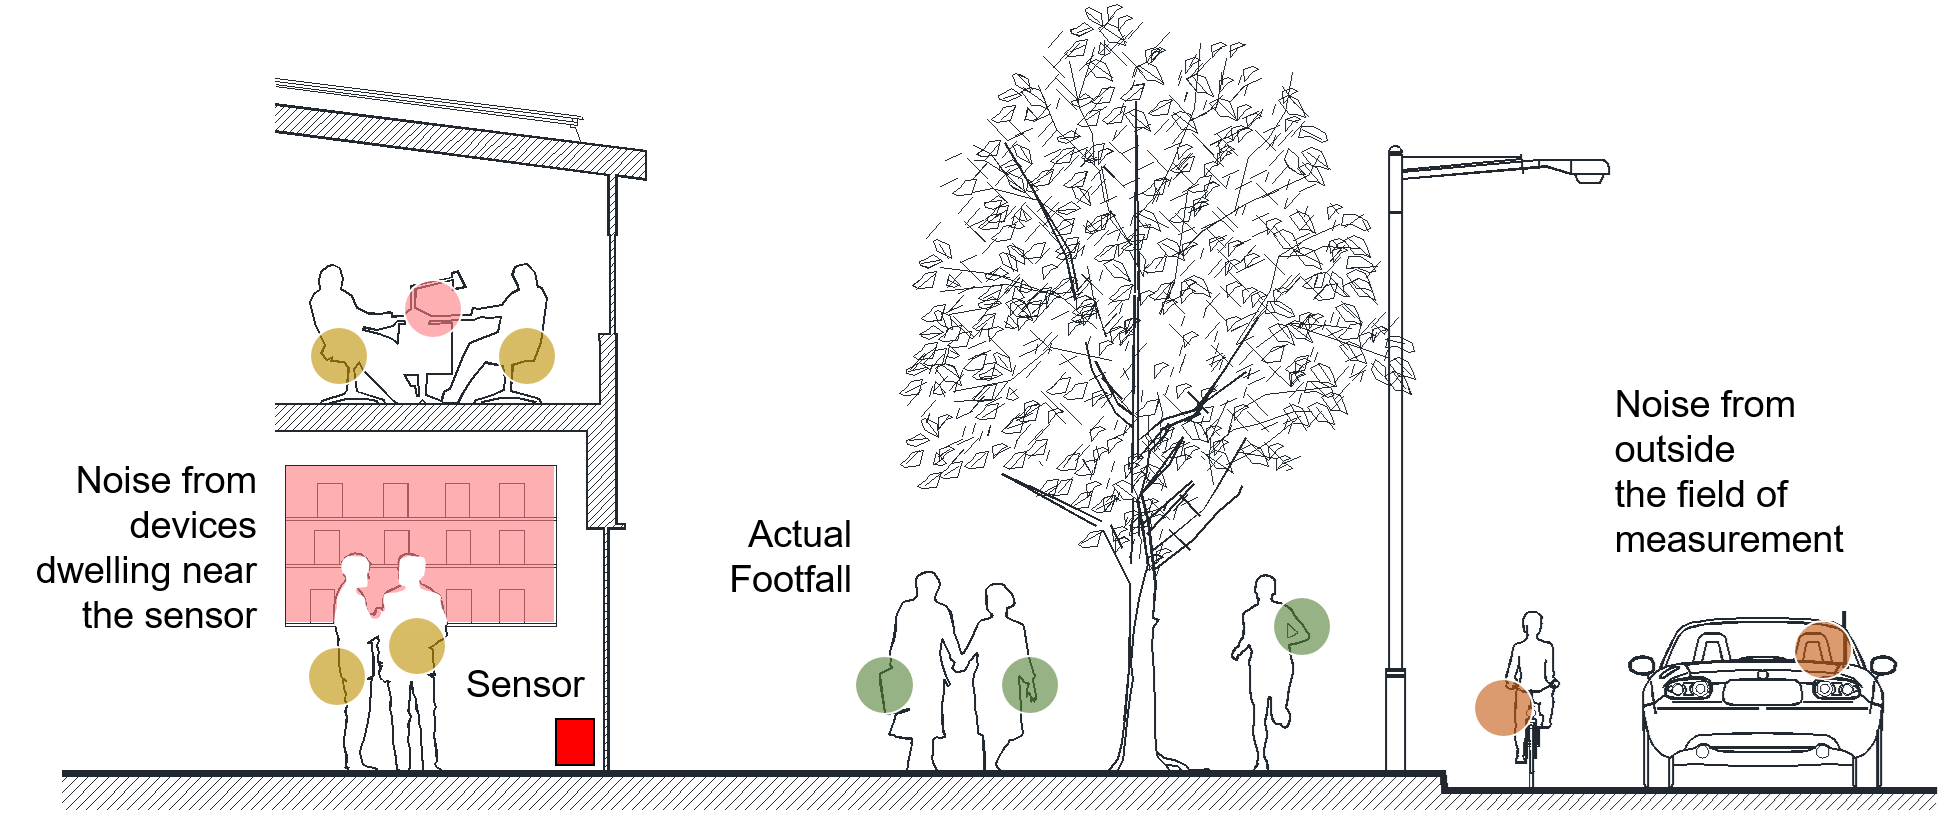
\includegraphics{images/sss.png}
  \caption{Cross section showing a typical installation of Smart Street Sensor in a retail frontage.}
  \label{figure:collection:sss:typical}
\end{figure*}

Due to the scale and the commercial nature of the project, the sensors collect fewer data per probe than the previous experiments.
The information collected by the Smart Street Sensors are the 5 minute interval when the probe request was collected, hashed MAC addresses and signal strength.
The probe requests within the same five minute intervals are aggregated by the MAC address, hence the signal strengths are aggregated to the minimum signal strength reported. 
Due to the longitudinal nature of the project, the data collection methods have changed over time as well.
The hardware was upgraded with more capabilities in early 2016, the interval they reboot at was adjusted several times in 2017, and finally, due to the MAC randomisation problem accentuated in the later part of 2017, the signal strength aggregation was changed from minimum to maximum in March 2018.
Essentially, the data have changed over time and we need to consider the changes while devising the methodologies for cleaning the data.
